


% Grundlegendes "Story Telling":
% Herstellung eines Zellkultur-Sensor Systems für die Messung von Aktionspotentialen
% --> Inkjet printing
% --> Tintenpräparation
% --> Galvanisierung
% --> Aerosol-Jet für PDOT pillars
% --> Tintenpräparation
% --> Aufbau mit den 3 Druck Systemen in die Theorie
% Leider gebremst bzw Abgebrochen wegen Verbindungsproblemen aufgrund gebrochener Netzwerkkabel im Druckkopf 

% Etablierung eines optimalen Workflows für die Herstellung von Lennarts Flow-Rate-Sensor:
% Auflösung der Druckstrukturen für Kanal und Passivierung
% --> Keyence-Auswerung
% Entfernung des Mikrofilms für freie Elektroden 
% --> Folie 
% --> Messung vor/nach Behandlung mit Schwefelsäure
% Kanal mit Fittings Haftung von beidem aufeinander
% --> Haftung an den Seiten der Fittings offenbar zu gering
% Deswegen Kanal mit zylindrischen Inlets 200µm??? radial größer als Schlauchdurchmesser
% --> ?
% Bonding
% --> ? 
% Sensorperformance
% --> ? Kalibrierung, CV, Impedanz

\subsection{Druckerauflösung}
\subsubsection{Teststrukturen}
Um die Auflösungslimits des Stereolithografen zu evaluieren, wurden verschiedene Teststrukturen designt (Abb. \ref{fig:ResolutionV1}). Diese bestanden aus pixelausgerichteten Kanälen mit den Breiten \SIlist{15; 30; 60; 90; 120; 150}{\micro \meter}, Quadraten aus einem Vielfachen der Auflösung (\SI{30}{\micro\meter} x \SI{30}{\micro\meter}, \SI{60}{\micro\meter} x \SI{60}{\micro\meter},...,\SI{240}{\micro\meter} x \SI{240}{\micro\meter}), sowie denselben vorhergenannten Quadraten mit einem zusätzlichen Pixel diagonal an den äußeren Ecken.

\begin{figure}[!h]
    \centering
    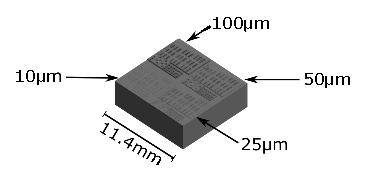
\includegraphics[width=\linewidth]{img/ResolutionV1.eps}
    \caption{Testdruck für die Auflösungsevaluation mit einem 2x2 Array derselben Struktur in den Layerhöhen \SI{10}{\micro\meter}, \SI{25}{\micro\meter}, \SI{50}{\micro\meter} und \SI{100}{\micro\meter} auf einem \SI{3}{\milli\meter} hohen Quader mit quadratischer Grundfläche (Kantenlänge \SI{11.4}{\milli\meter}).}
    \label{fig:ResolutionV1}
\end{figure}

Des Weiteren wurden verschiedene - ebenfalls pixelausgerichtete - Axondioden-Strukturen getestet. Bei solchen Kanälen wurden einerseits die Kanalbreite (\SIrange{1}{3}{px}) und -länge (\SIrange{3}{5}{px}) in den Durchgängen zwischen einzelnen Dioden und andererseits die Größe der dreieckigen Dioden (3-5 Stufen) variiert. Zu Testzwecken wurden außerdem um \SI{45}{\degree} gedrehte Kanäle, Quadrate und Wells in das Layout aufgenommen, jedoch aus Zeitgründen nicht ausgewertet.

Das fertig erstellte Layout wurde dann auf einem Quader mit den Maßen \SI{11.4}{\milli\meter} x \SI{11.4}{\milli\meter} x \SI{3}{\milli\meter} mit den Höhen \SI{10}{\micro\meter}, \SI{25}{\micro\meter}, \SI{50}{\micro\meter} und \SI{100}{\micro\meter} extrudiert. Dieses Werkstück diente nun als Standard für 3D-Drucke mit zwei verschiedenen Resins (MPC und PEGDA) auf den Slicerhöhen \SIlist{10; 25; 50; 100}{\micro\meter}.\\

Um die Druckbarkeit einer einlagigen Passivierungsschicht auf den Sensorchip mit definierter Öffnungsbreite und den zurückbleibenden Resin-Mikrofilm auf der Öffnung zu evaluieren, wurde eine zweite Teststruktur designt (Abb. \ref{fig:ResolutionLennart}). Hier wurden sowohl rechteckige Öffnungen verschiedener Breiten und Längen, als auch dieselben Öffnungen mit einer angeschlossenen Aufweitung auf beiden Seiten getestet. Diese Strukturen wurden einerseits pixelausgerichtet und anderseits um \SI{45}{\degree} gedreht mit \SI{10}{\micro\meter} und \SI{20}{\micro\meter} Höhe auf einen Mikroskopieträger gedruckt. Die Kanaldimensionen wurden mit folgenden Parametern designt:
\begin{itemize}
    \item \textbf{Breite:} \SIlist{30;60;90;120;150;210;300;510}{\micro\meter}
    \item \textbf{Länge:} \SIlist{300;600;900}{\micro\meter}
    \item \textbf{Endseiten:} Flache Enden, Endaufweitung mit Breite \SI{600}{\micro\meter} und Länge \SI{300}{\micro\meter}
\end{itemize}

\begin{figure}[!h]
    \centering
    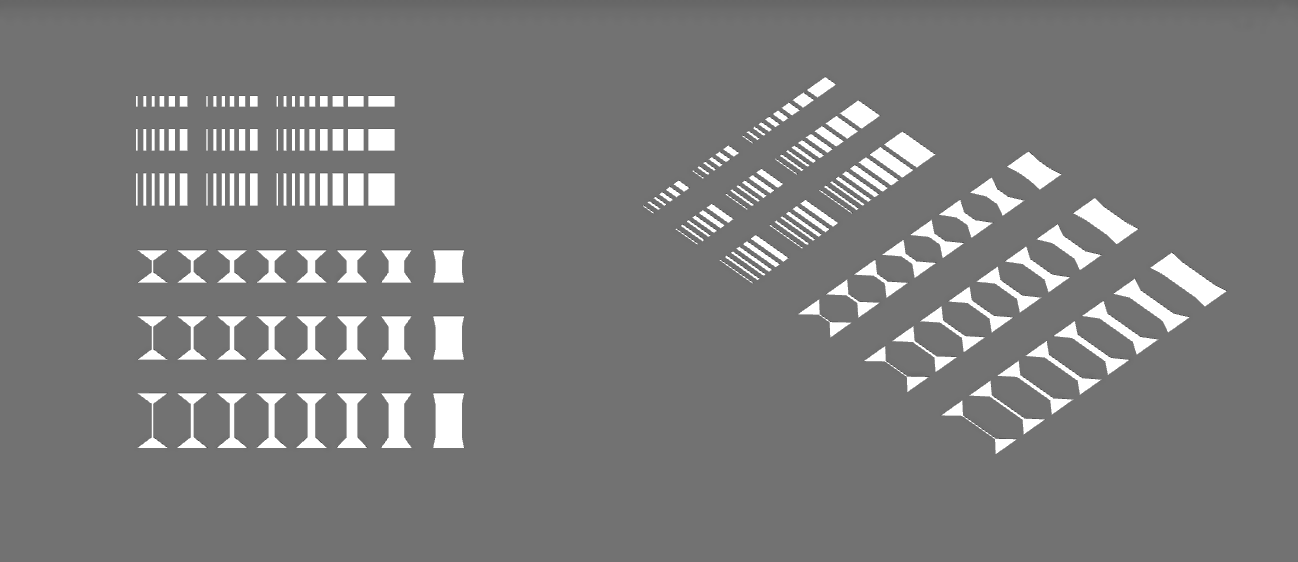
\includegraphics[width=\linewidth]{img/ResolutionLennart.png}
    \caption{Teststrukturen für die Bestimmung der Auflösung von Ein-Lagen-Drucken, sowie vorhandener Mikrofilme.}
    \label{fig:ResolutionLennart}
\end{figure}

\clearpage
\subsubsection{Auflösung}

\begin{figure}[!h]
    \centering
    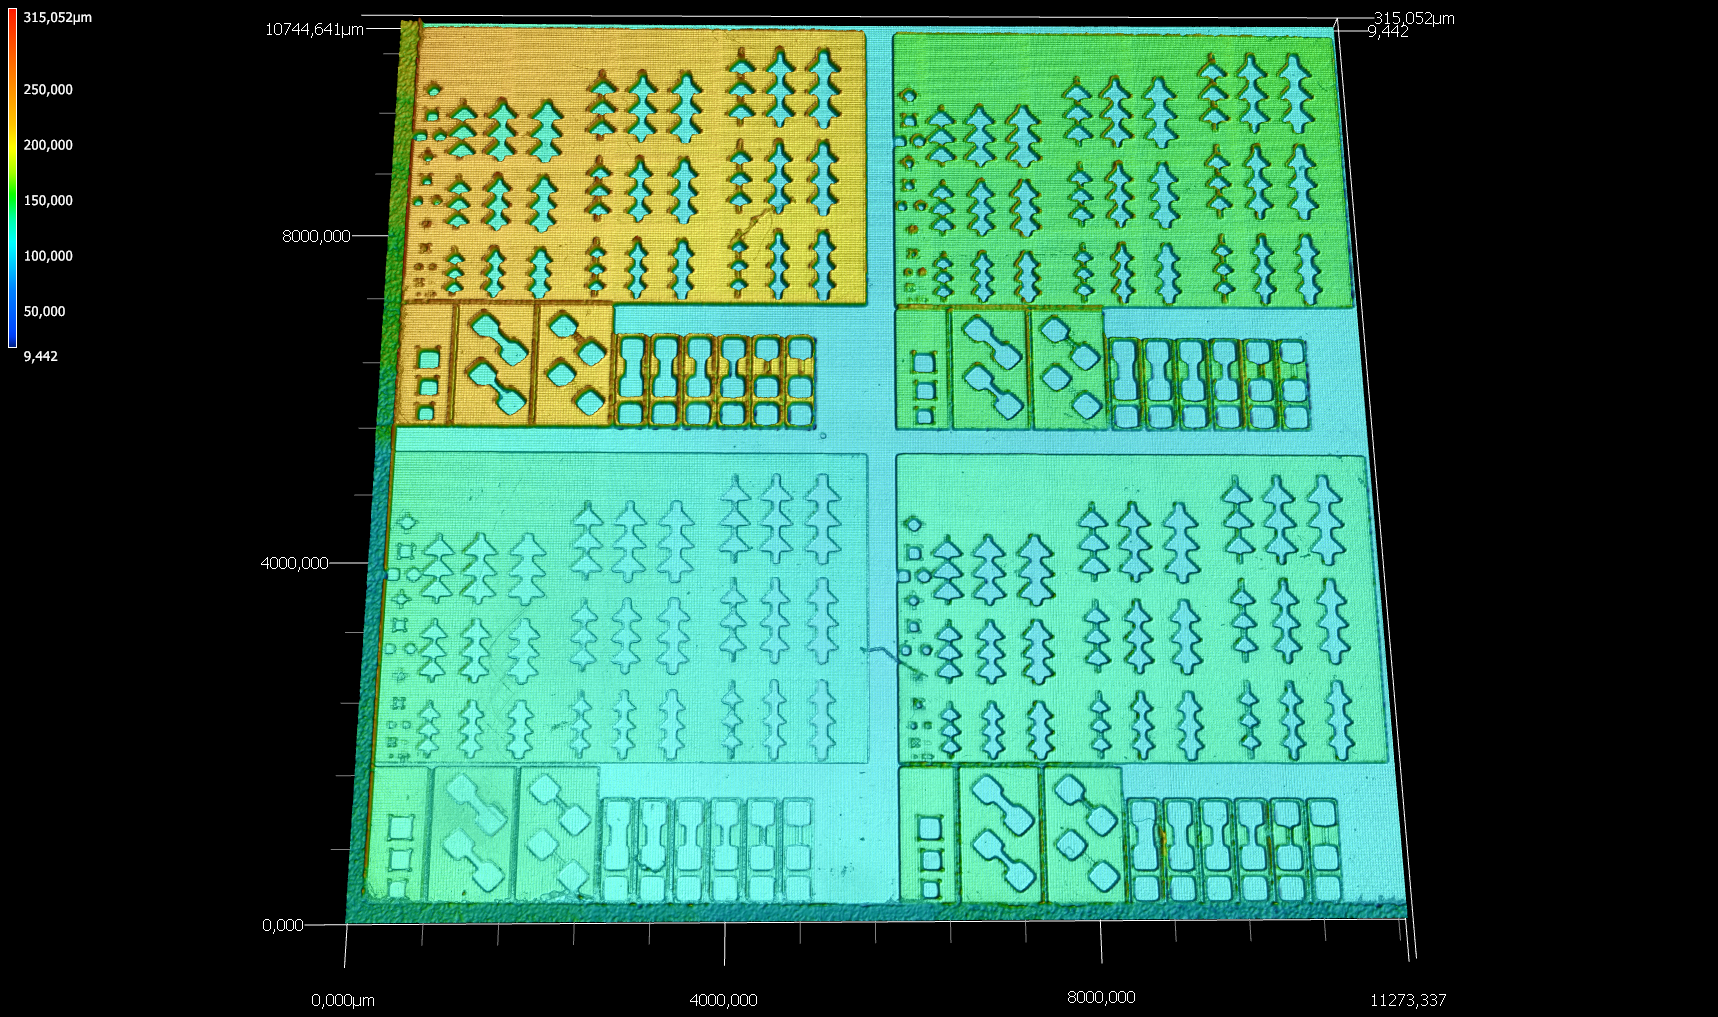
\includegraphics[width=\linewidth]{img/PEGDA-10um-3d.png}
    \caption{Oberflächenprofil des PEGDA Werkstücks mit \SI{10}{\micro\meter} z-Auflösung.}
    \label{fig:Surface_PEGDA_10um}
\end{figure}

Die Oberflächenvermessung der Testdrucke sollte nun die laterale und Tiefenauflösung des Druckers charakterisieren. Bereits vor der Durchführung bestand die Annahme, dass die höhere Viskosität des MPC gegenüber des PEGDA Resins die Auflösung negativ beeinflussen könnte, da mehr Material in den Strukturöffnungen diffusiv ausgehärtet würde.
Dies bestätigt ein Vergleich der Einzellagenstrukturen mit \SI{10}{\micro\meter} Höhe.

Der PEGDA-Druck (Abb. \ref{fig:PEGDA_10um}) zeigt eine im Durchschnitt höhere Tiefe als ursprünglich angepeilt. Das legt den Schluss nahe, dass zu wenig Resin in der Tiefe quervernetzt wird. Gleichzeit erhöht diese geringere Aushärtung die laterale Auflösung im Vergleich zu MPC. Diese Annahme wird qualitativ dadurch gestützt, dass die MPC Breiten konträr zum PEGDA zumeist unter der nominellen Breite liegen.

Im Gegensatz zum PEGDA-Druck fehlen bei MPC (Abb. \ref{fig:MPC_10um}) bereits die \SI{15}{\micro\meter} breiten Kanäle komplett und die Tiefen nähern sich erst ab \SI{150}{\micro\meter} Strukturbreite (also 5 Pixeln) den angepeilten \SI{10}{\micro\meter}. Dasselbe Bild ergibt sich für die ausgewerteten Höhen von \SIlist{25;50}{\micro\meter} unter Punkt \ref{appendix}. Zusätzlich sind bei den 3D-Profilometeraufnahmen der PEGDA-Drucke (im Gegensatz zu MPC) die Grenzen der einzelnen Mikrospiegel sichtbar.
Daraus kann man einerseits eine allgemein höhere Auflösung mit diesem Resin schließen, andererseits scheint eine homogene Oberfläche der Strukturen nicht gegeben zu sein. Wir vermuten, dass die Pixelkanten durch die Überlappung von aneinanderliegenden Linsen verursacht werden. \\
\clearpage
\begin{figure}[!h]
    \centering
    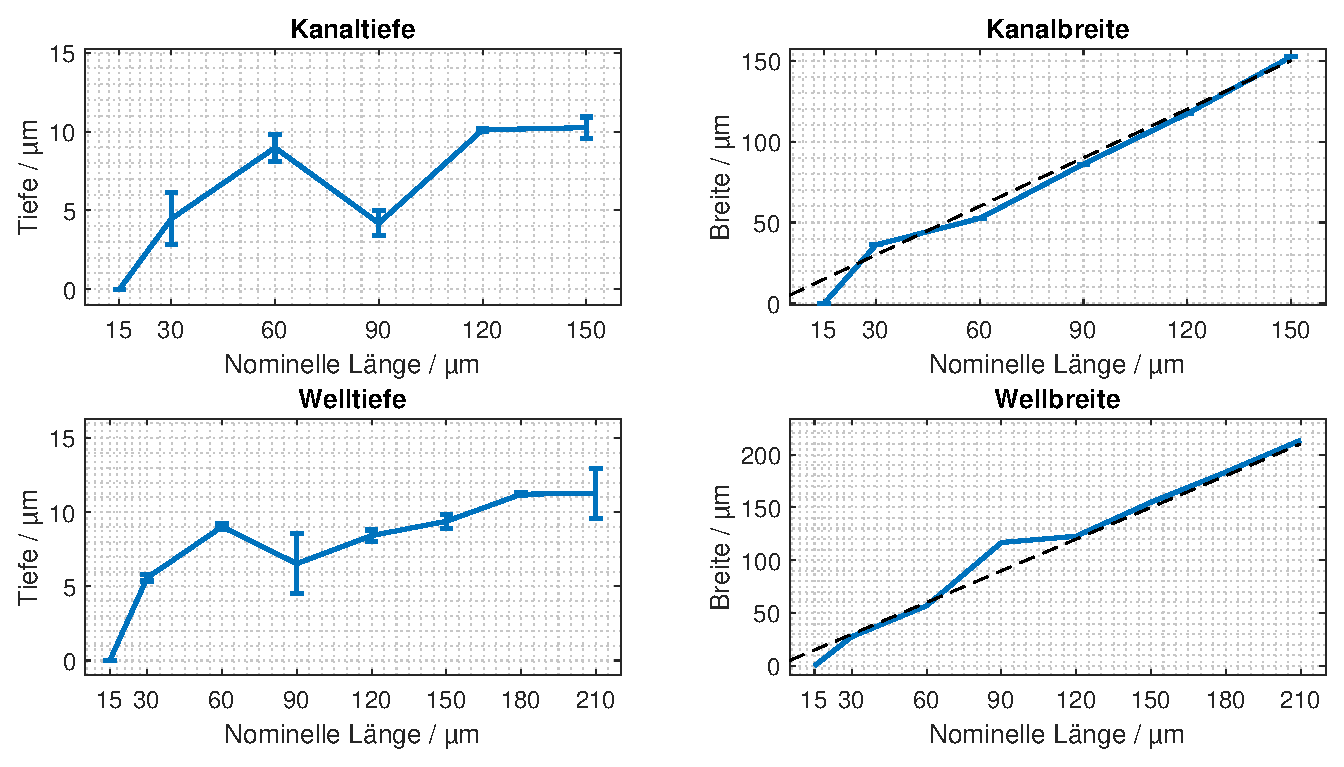
\includegraphics[width=\linewidth]{plot/10um_SL_ResolutionV1.eps}
    \caption{Profilometrie des \SI{10}{\micro\meter}-Einzellayers aus MPC. Da in den Kanalbreiten keine laterale Varianz messbar war (siehe Fehlerbalken Kanalbreite), wurden Fehlerbetrachtungen bei den Breitenprofilen vernachlässigt. (\textcolor{black}{\textbf{- - -}}) gibt die ideal gedruckte Breite an.}
    \label{fig:MPC_10um}
\end{figure}

\begin{figure}[!h]
    \centering
    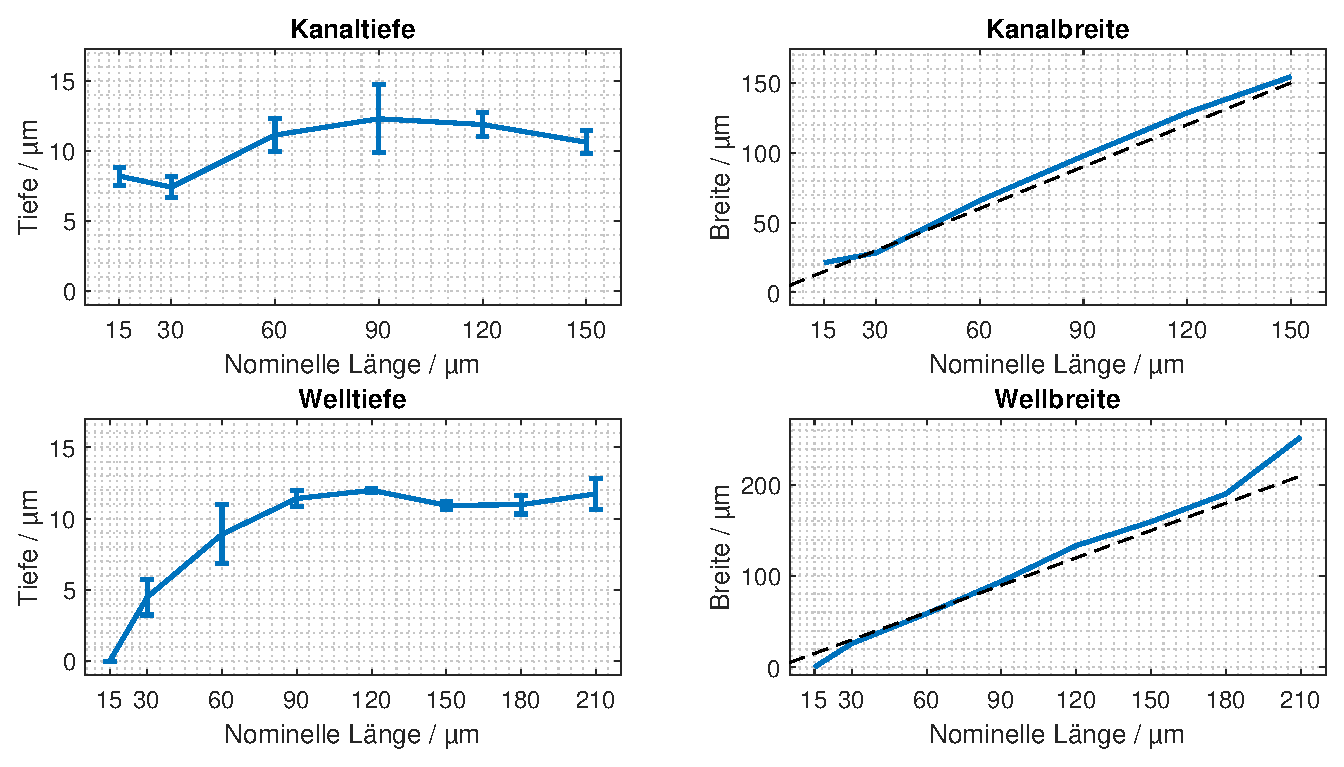
\includegraphics[width=\linewidth]{plot/PEGDA_10um_SL_ResolutionV1.eps}
    \caption{Profilometrie des \SI{10}{\micro\meter}-Einzellayers aus PEGDA. (\textcolor{black}{\textbf{- - -}}) gibt die ideal gedruckte Breite an.}
    \label{fig:PEGDA_10um}
\end{figure}
\clearpage

Als weiterer Punkt der Druckercharakterisierung wurde der Einflusses von Lichtintensität auf das Druckergebnis bestimmt. Aus Zeitgründen wurde hierbei die Leistung bei dem \SI{50}{\micro\meter}-Einzellayer der MPC-Drucke einmalig von \SI{125}{\percent} auf \SI{100}{\percent} - also um \SI{20}{\percent} - verringert. Die Exposurezeit von \SI{1}{\second} wurde konstant gehalten. Mit der verringerten Lichtleistung sollte dem diffusiven Quervernetzen des Resins an ungewollten Stellen entgegengewirkt werden.

Qualitativ kann man aus den Auswertungen von \SI{50}{\micro\meter} bei \SI{125}{\percent} (Abb. \ref{fig:MPC_50um}) und \SI{100}{\percent} (Abb. \ref{fig:MPC_50um_100perc}) erschließen, dass insbesondere \SIlist{15;30}{\micro\meter} Kanäle mit geringerer Leistung überhaupt erst aufgelöst werden können.

Aus ungeklärter Ursache sind die mit geringerer Leistung gedruckten Strukturen näher an der nominellen Tiefe von \SI{50}{\micro\meter}, als diejenigen der Standardleistung. Unseren bisherigen Ergebnissen nach, müssten im Druck mit höherer Energie durch erhöhte diffusive Strahlung mehr Resin quervernetzen und die Tiefe somit nachhaltig verringert werden.

\begin{figure}[!h]
    \centering
    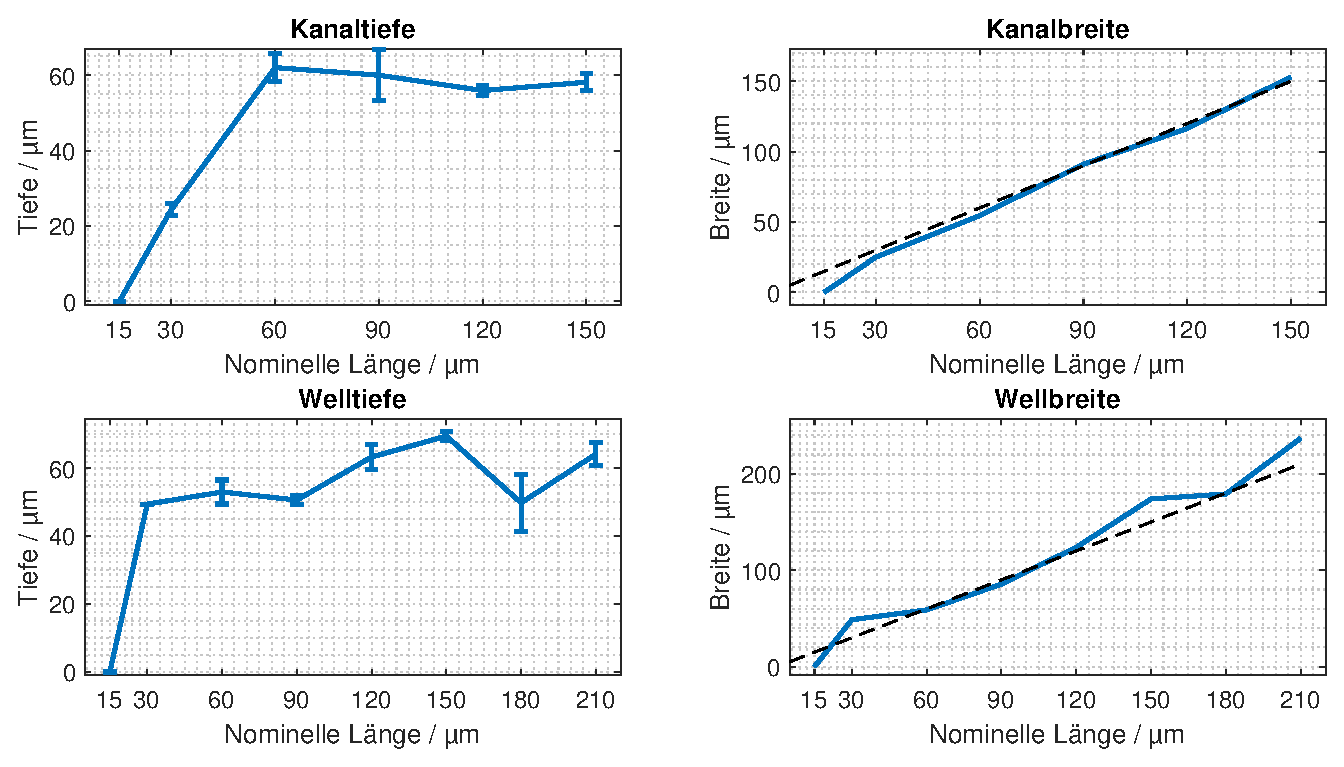
\includegraphics[width=\linewidth]{plot/50um_SL_ResolutionV1.eps}
    \caption{Profilometrie des \SI{50}{\micro\meter}-Einzellayers aus MPC. (\textcolor{black}{\textbf{- - -}}) gibt die ideal gedruckte Breite an.}
    \label{fig:MPC_50um}
\end{figure}
\clearpage
\begin{figure}[!h]
    \centering
    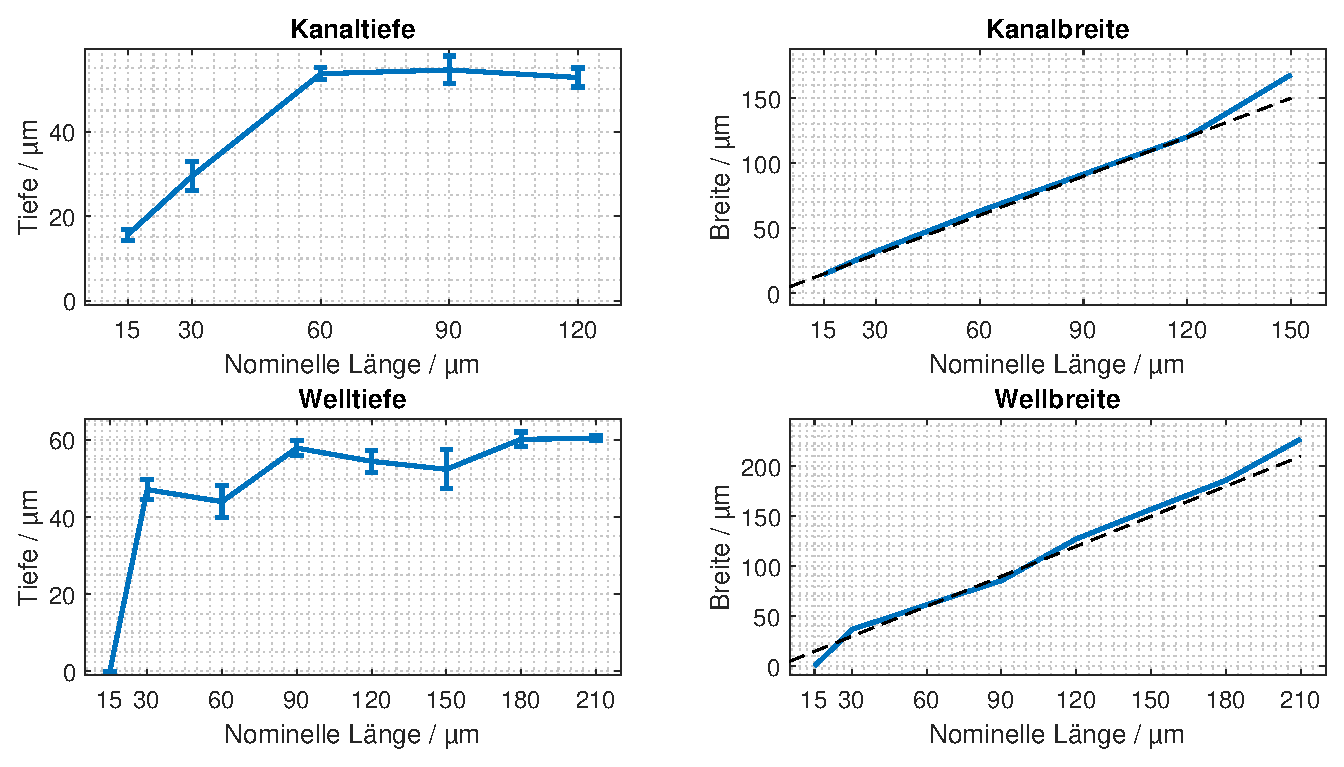
\includegraphics[width=\linewidth]{plot/50um_100perc_SL_ResolutionV1.eps}
    \caption{Profilometrie des \SI{50}{\micro\meter}-Einzellayers aus MPC mit \SI{100}{\percent} (also \SI{20}{\percent} weniger) Leistung.  (\textcolor{black}{\textbf{- - -}}) gibt die ideal gedruckte Breite an.}
   \label{fig:MPC_50um_100perc}
\end{figure}

\subsection{Passivierungsstrukturen}

Im Anschluss an die Auflösungstests, sollte eine auf einen silanisierten Glaschip gedruckte Passivierungsschicht des Druckers etabliert werden. Auf Basis der besseren Druckergebnisse des PEGDA Resins, wurden die folgenden Tests ausschließlich mit diesem Harz durchgeführt. In diesem Schritt sollte auf der einen Seite getestet werden, welche Öffnungsbreiten noch realisiert werden können. Auf der anderen Seite sollte die Vermutung eines Resin-Mikrofilms in der Öffnung bestätigt und entsprechende Gegenmaßnahmen ergriffen werden.

Zu diesem Zweck wurde zuerst eine Alignmentstruktur auf den Picker gedruckt, an dem der Glaschip später ausgerichtet werden sollte. Dieser wurde dann mittels Kapton auf dem gesäuberten Picker befestigt. Anschließend wurde die Passivierung mit einem Offset von \SI{0.52}{\milli\meter} auf den Chip gedruckt. Nach unterschiedlichen Behandlungsdauern mit Isopropanol in einem Ultraschallbad, wurden die Drucke dann im Profilometer vermessen. Dort zeigte sich, dass eine Behandlung von \SIlist{5;10;30}{\minute} bei Layerhöhen von \SIlist{10;20}{\micro\meter} keine Öffnung produzieren konnte.

Durch die Vorarbeiten anderer Studenten motiviert, wurde der Picker und die Alignmentstruktur mit einer schwarzen Mülltüte überklebt. Das Vorgehen basiert auf der Annahme, dass der graue Aluminiumpicker die Belichtung in das umliegende Resin zu stark reflektiert und es so mitaushärtet. Mit dem modifizierten Picker wurden die obigen Experimente noch einmal durchgeführt.

Die Ergebnisse nach verschiedenen Behandlungen (\SIlist{5;10;30}{\minute}) im Ultraschallbad sind in Abbildung \ref{fig:Microfilm} dargestellt. Hier sind bei größeren Strukturen deutliche Öffnungen sichtbar, sodass mit Vernachlässigung der kleinsten Öffnung minimale Parameter bestimmt werden können. Sowohl für die flachen, als auch für die aufgeweiteten Enden ergibt sich eine minimale Breite von \SI{240}{\micro\meter}. Die Länge der Öffnung scheint eine untergeordnete Rolle zu spielen und wurde in einem Bereich von \SIrange{300}{900}{\micro\meter} validiert.

Ein signifikanter Einfluss der aufgeweiteten Enden auf die Strukturöffnung gegenüber dem recheckigen Standard konnte nicht gezeigt werden. Auch scheint eine Verlängerung der Ultraschallbehandlung das Druckergebnis nicht zu verbessern. Im Gegenteil, bei schlechter Silanisierungsqualität bzw. allgemein schlechter Haftung des Drucks auf dem Glaschip löste sich in manchen Fällen die Passivierung wieder.

\begin{figure}[htb!]
\begin{subfigure}[l]{0.3\linewidth}
\centering
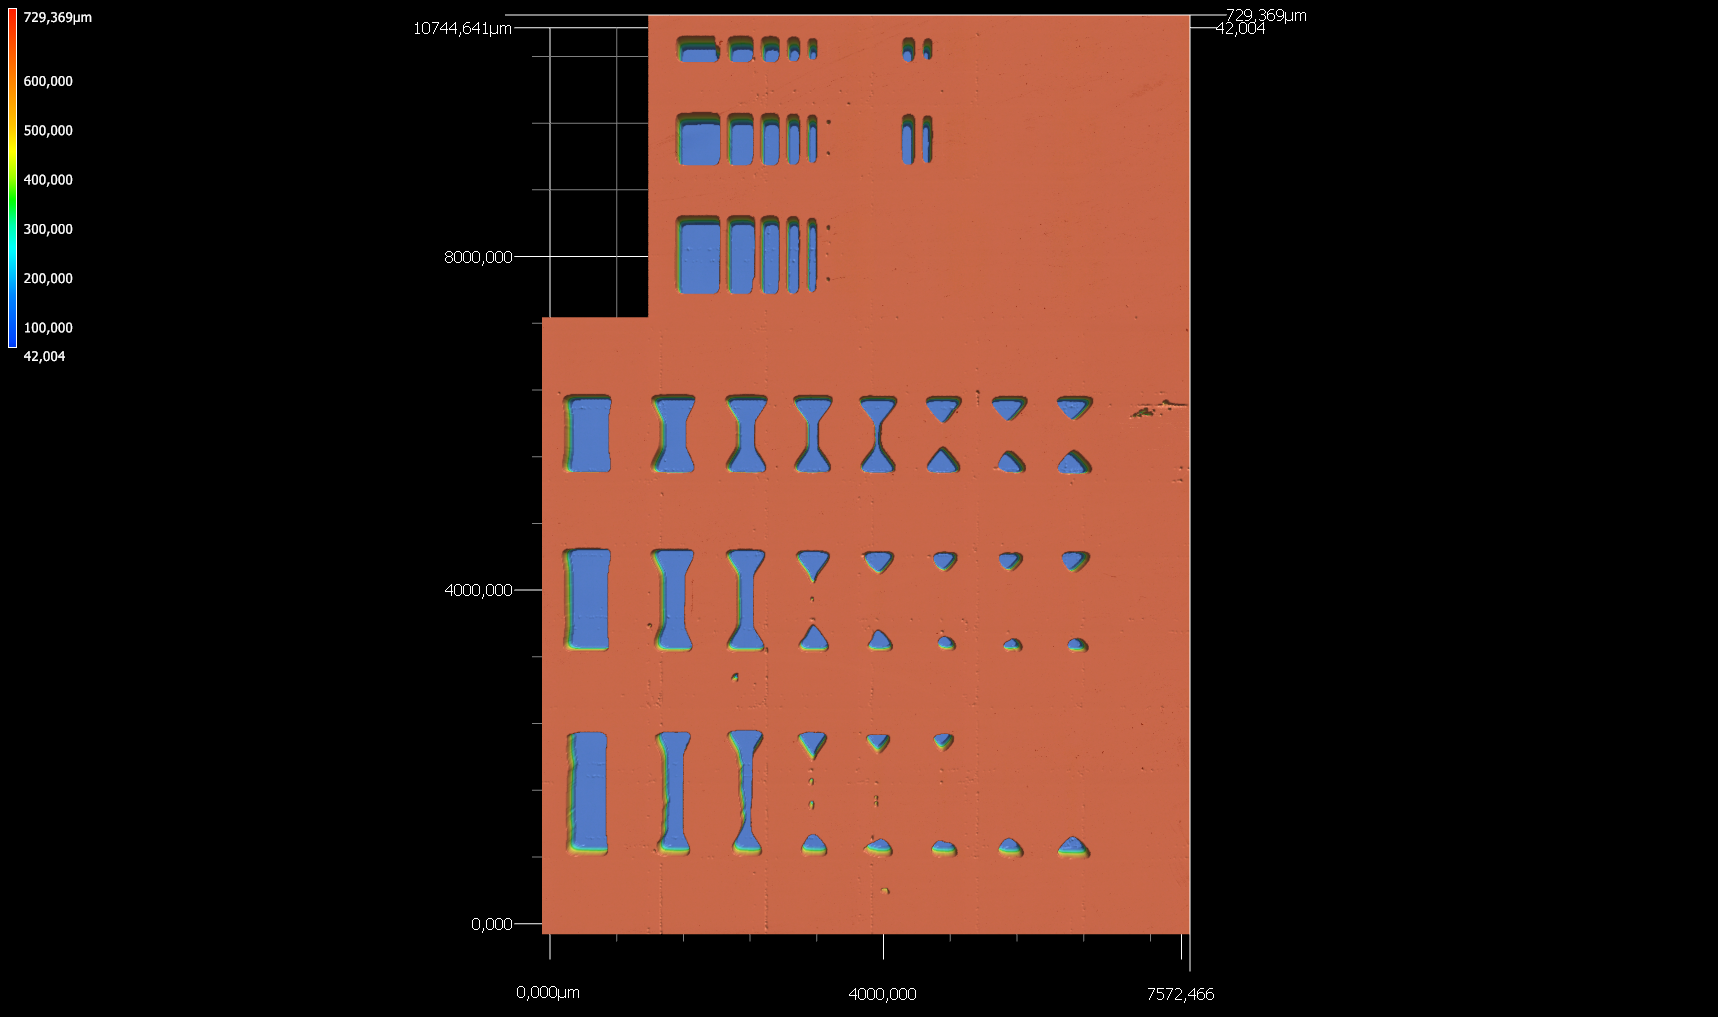
\includegraphics[clip, trim=0 0mm 50 0, width=\linewidth]{img/10um-05min-Folie-3d.png}
\subcaption{\SI{5}{\minute} Ultraschallbad}
\end{subfigure}%
\hspace{6mm}
\begin{subfigure}[c]{0.3\linewidth}
\centering
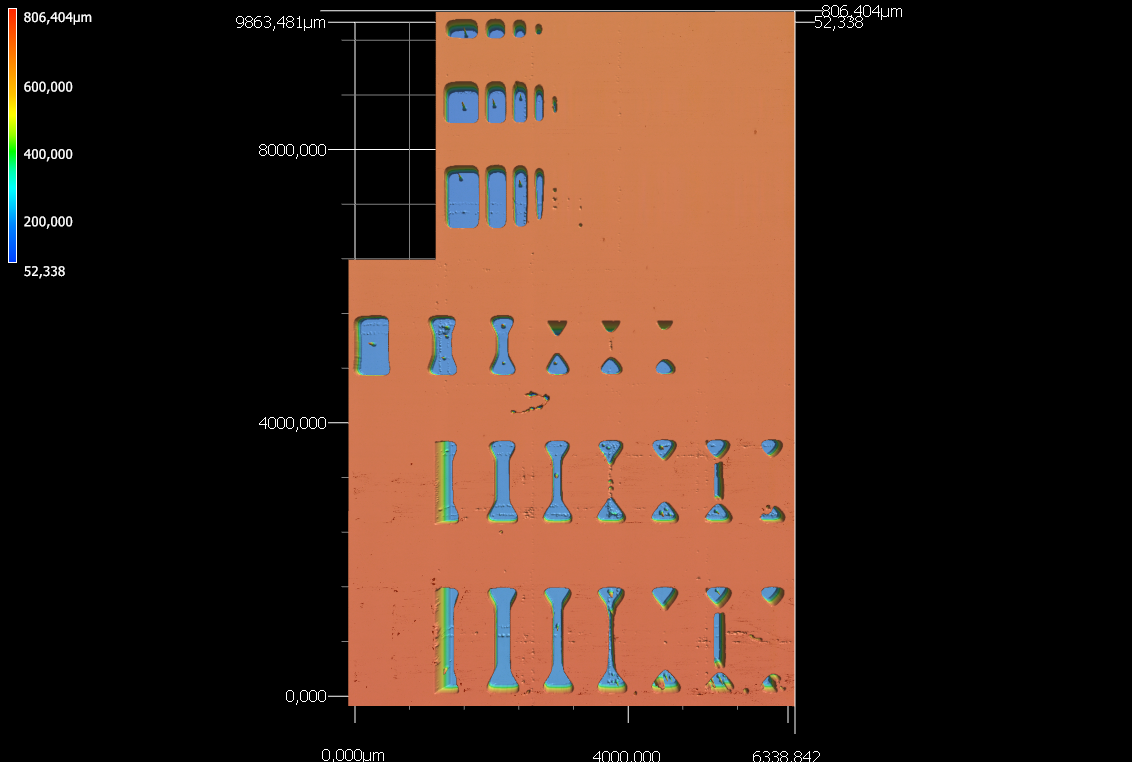
\includegraphics[clip, trim=0 0mm 0 0,width=\linewidth]{img/10um-10min-Folie-3d.png}
\subcaption{\SI{10}{\minute} Ultraschallbad}
\end{subfigure}%
\hspace{6mm}
\begin{subfigure}[r]{0.3\linewidth}
\centering
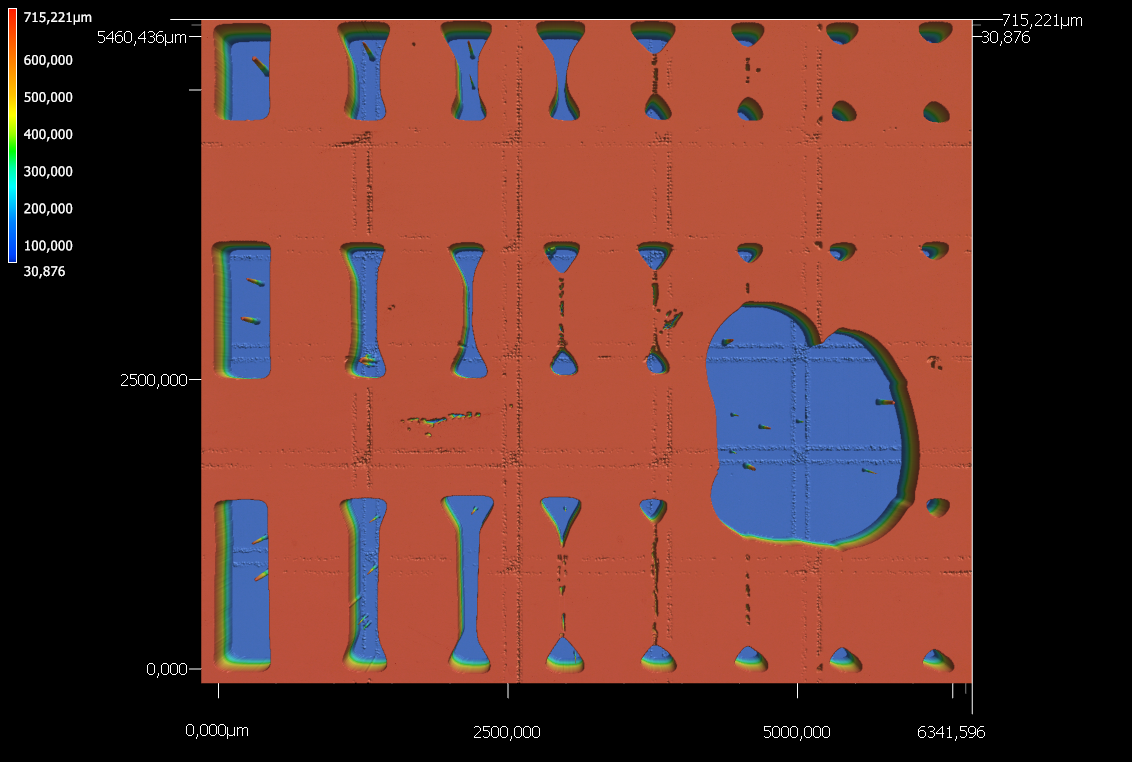
\includegraphics[clip, trim=0 0mm 0 0,width=\linewidth]{img/10um-30min-Folie-3d.png}
\subcaption{\SI{30}{\minute} Ultraschallbad}
\end{subfigure}
\caption{Oberflächen der \SI{10}{\micro\meter} passivierten Chips nach der Modifizierung des Pickers mit schwarzer Folie.}
\label{fig:Microfilm}
\end{figure}



\subsection{Bonding}

\begin{wrapfigure}[14]{r}{0.4\linewidth}
    \centering
    \vspace{-16pt}
    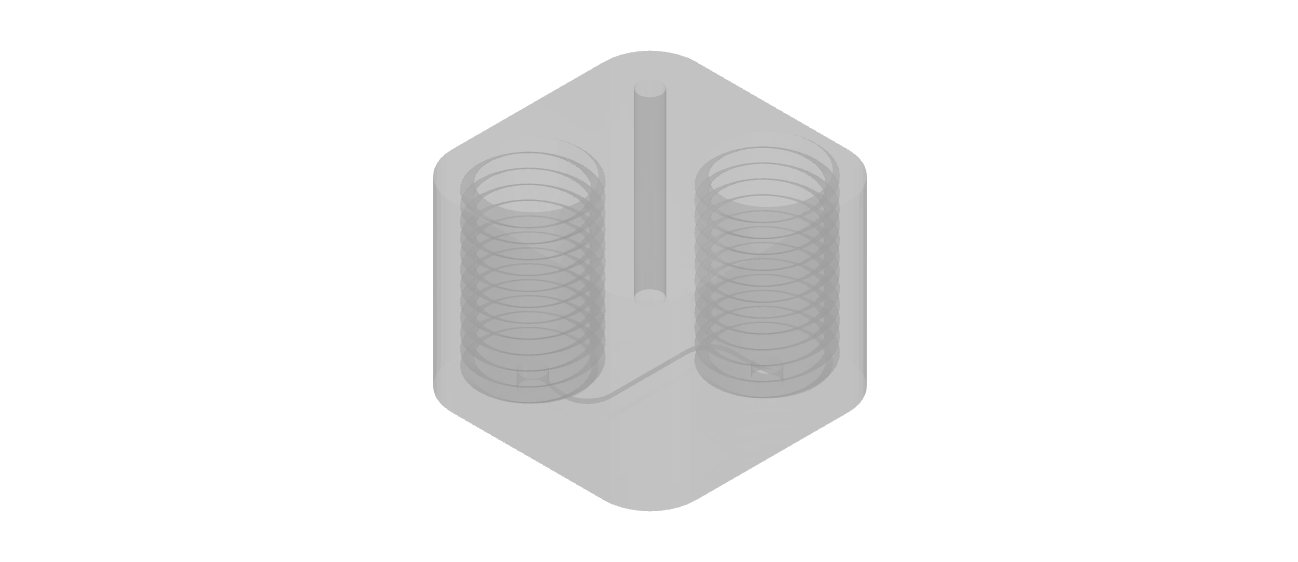
\includegraphics[clip,trim=11mm 2 10mm 3,width=1.15\linewidth] {img/Fitting.png}
    \caption{Mikrofluidikkanal mit 1/4\dq-28 Feingewinde für Fittings}
    \label{fig:Mikrofluidik_Gewinde}
\end{wrapfigure}
Als nächster Schritt im Workflow wurde die Verbindung von einer designten Mikrofluidik mit dem passivierten Sensorchip untersucht. Dafür wurden zuerst simple Kanäle mit Schraubverbindungen für Fittings der Elveflow- und Fluigent-Systeme designt (Abb. \ref{fig:Mikrofluidik_Gewinde}). Sowohl die Kanäle, als auch die passivierten Chips wurden vor dem Aushärten im Polymerisationsgerät in einer Schraubzwinge verpresst und so permanent verbunden.

In unseren Versuchen konnte in einem anschließenden Drucktest mit flüssigkeitsgefüllten Schläuchen keine Dichtigkeit nachgewiesen werden. Bei Drücken über \SI{20}{\milli\bar} trat an den Seiten der Inlets Flüssigkeit aus und der Kanal löste sich von der Passivierung. Bei zukünftigen Designs könnte ein zusätzlicher Abstand der Inlets zum Rand des Chips und somit mehr Klebefläche ein Lösungsansatz sein. \\

\begin{figure}[!ht]
    \centering
    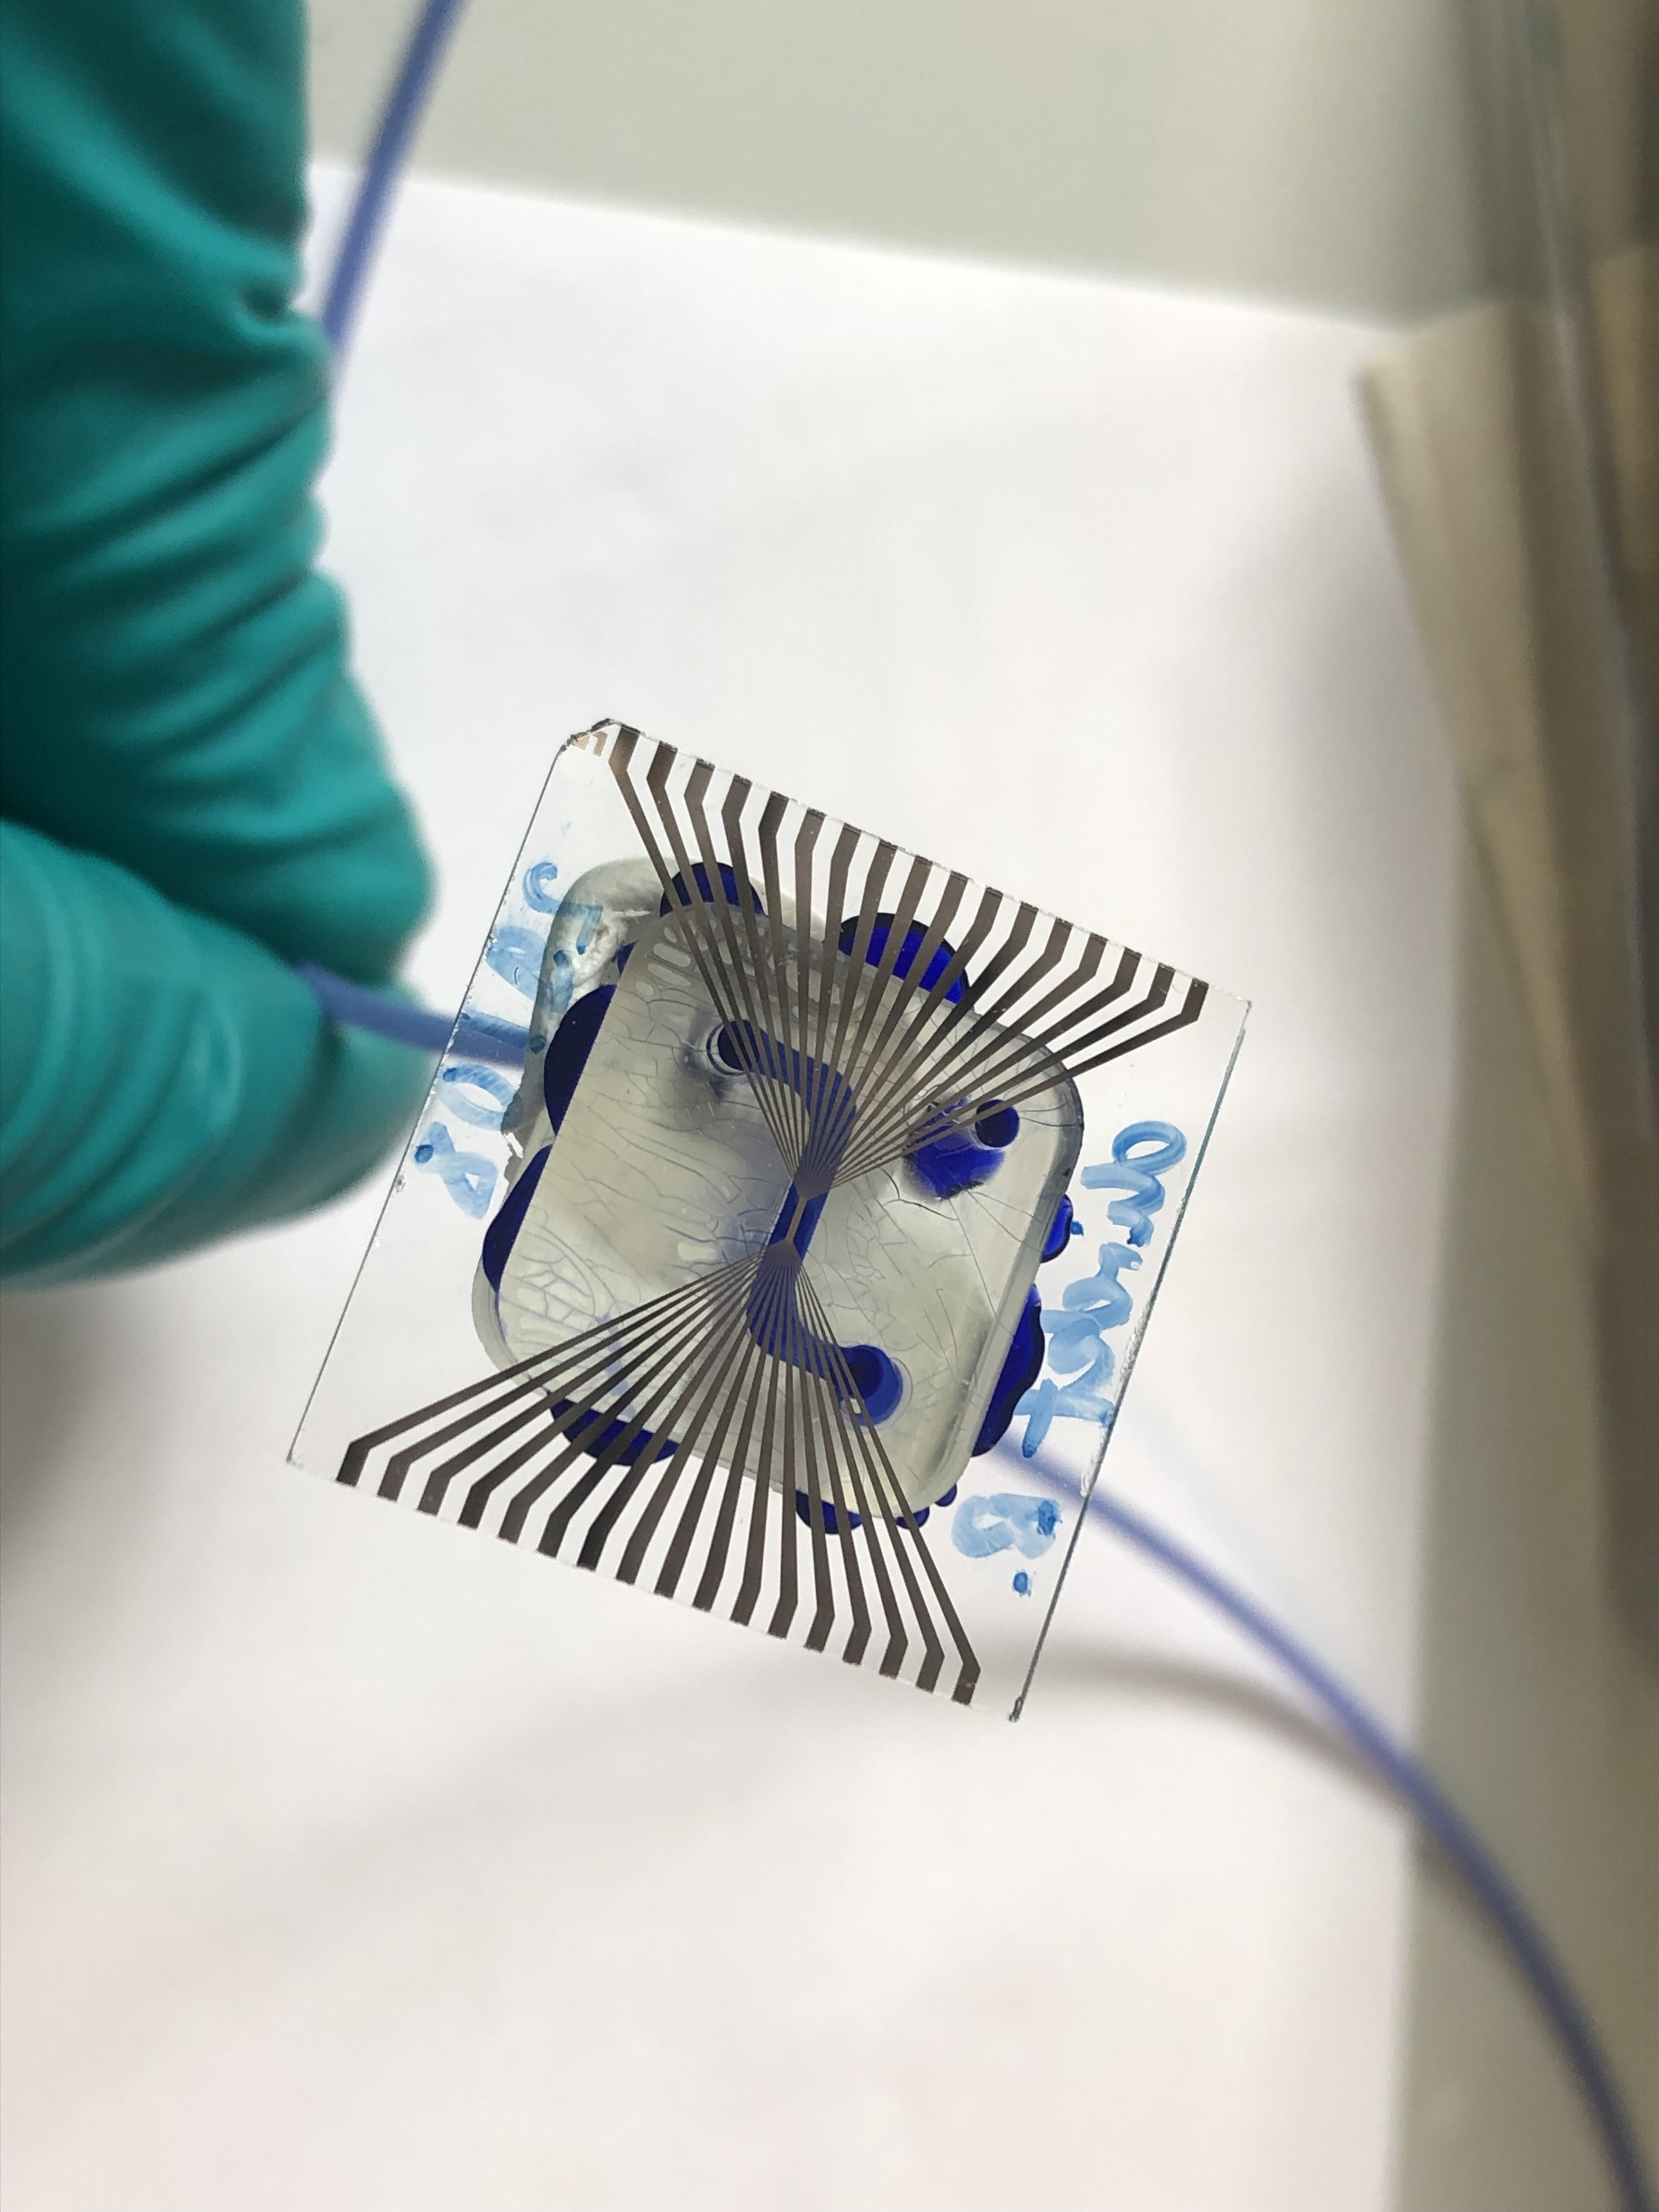
\includegraphics[trim=75 450 100 400mm, clip, width=1.0\textwidth]{img/MIKRORISS.jpeg}
    \caption{Undichte Mikrofluidik auf dem passivierten Sensorchip. Der Kanal wurde zur besseren Sichtbarkeit mit blauer Tinte angefärbt.}
    \label{fig:Mikrofluidik_undicht}
\end{figure}

Als weiterer Ansatz, um die Verbindungsqualität zu erhöhen, wurde ein Plasmacleaning der Werkstücke für \SI{0.7}{\minute} in O$_2$-Plasma - ähnlich zu einer PDMS - Fabrikationsmethode - getestet. Die ersten qualitativen Tests verliefen dahingehend ebenfalls negativ.\\

Ein zusätzlicher Faktor für die mangelnde Druckfestigkeit sind auch Risse an der Unterseite des Drucks. Deren Entstehung konnte im Verlauf des Praktikums nicht abschließend geklärt werden, vermutlich sind jedoch Spannungen innerhalb des Materials durch ungleichmäßige Polymerisation oder Schrumpfung verantwortlich.


\subsection{Elektrochemische Vermessung des Passivierungslayers}
Zusätzlich zu den Verbindungstests mit der Passivierung wurden auch die elektrochemischen Eigenschaften der Elektroden nach der Passivierung durch EIS und CV analysiert. Es wurde erwartet, dass bedeckte Elektroden eine höhere Impedanz und eine kleinere Hysterese im CV besitzen. Außerdem können vollkommen bedeckte Elektroden die charakteristischen Peaks eines Elektrolyten nicht anzeigen.

\begin{figure}[!htb]
\begin{subfigure}[l]{0.49\linewidth}
\centering
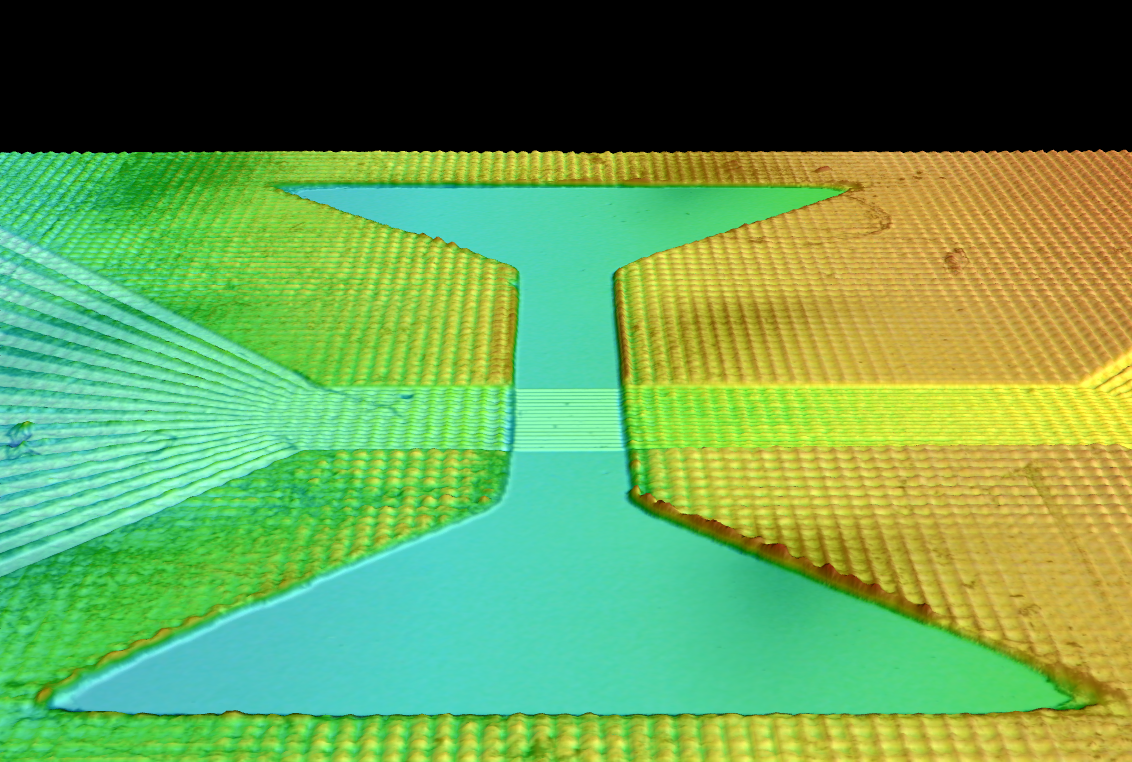
\includegraphics[trim=0 0mm 0 115,clip,width=\linewidth]{img/180mu.png}
\subcaption{\SI{180}{\micro\meter} Passivierung}
\end{subfigure}%
\hspace{6mm}
\begin{subfigure}[r]{0.49\linewidth}
\centering
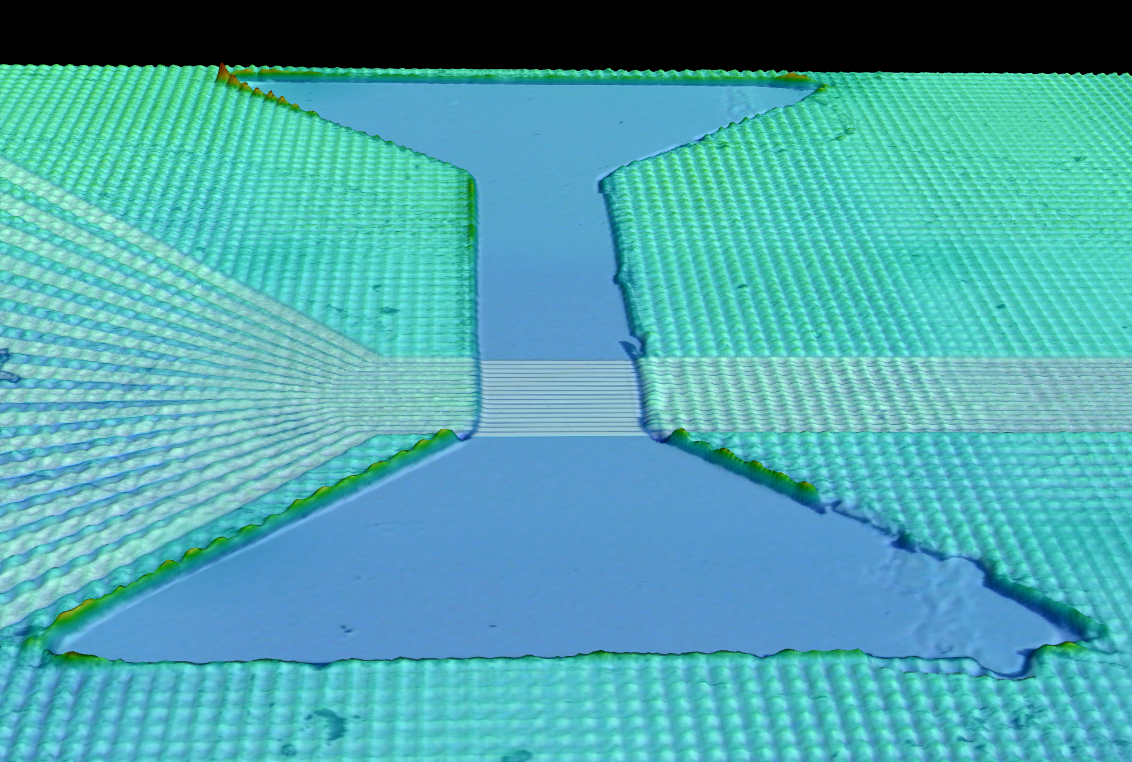
\includegraphics[trim=0 20mm 0 50,clip,width=\linewidth]{img/240um.png}
\subcaption{\SI{240}{\micro\meter} Passivierung}
\end{subfigure}
\caption{Passivierung der Elektrodenstrukturen nach der Behandlung mit \SI{13}{\percent}-iger Schwefelsäure}
\label{fig:passivierung}
\end{figure}

Im Zuge der Experimente wurden Elektrodenöffnungen mit \SIlist{180;210;240}{\micro\meter} Breite vermessen. In den Versuchen wurden CV und EIS der Elektroden vor und nach der Behandlung mit Schwefelsäure gemessen. Während der Reinigung mit 13\% Schwefelsäure, wurden 40 CV-Zyklen mit kurzgeschlossenen Elektroden durchgeführt.


\begin{figure}[!htb]
\begin{subfigure}[l]{0.31\linewidth}
\centering
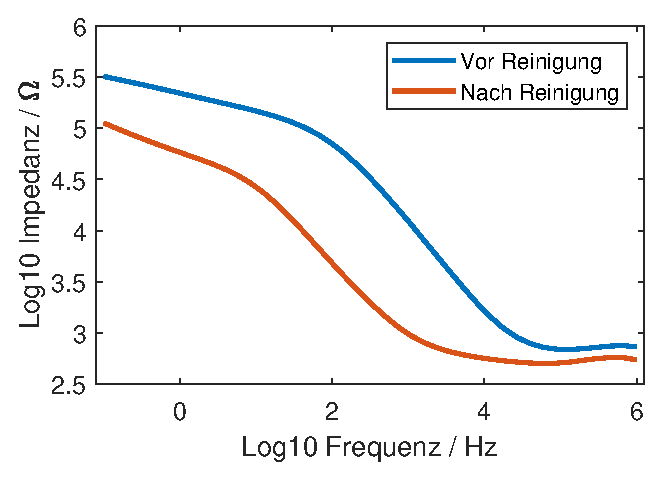
\includegraphics[trim=0 0mm 0 0,clip,width=\linewidth]{plot/EIS_180um.eps}
\subcaption{EIS vor und nach dem Reinigungszyklus}
\label{fig:EIS}
\end{subfigure}%
\hspace{4mm}
\begin{subfigure}[c]{0.31\linewidth}
\centering
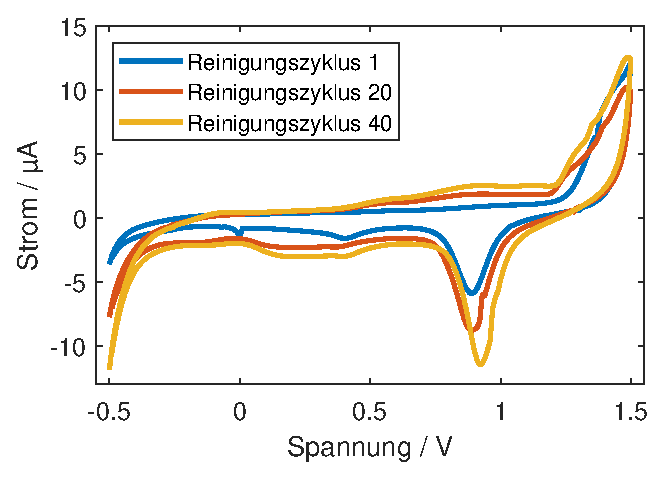
\includegraphics[trim=0 0mm 0 0,clip,width=\linewidth]{plot/Cleaning_180um.eps}
\subcaption{CV-Zyklen während der Elektrodenreinigung}
\label{fig:CV_reinigung}
\end{subfigure}%
\hspace{4mm}
\begin{subfigure}[r]{0.31\linewidth}
\centering
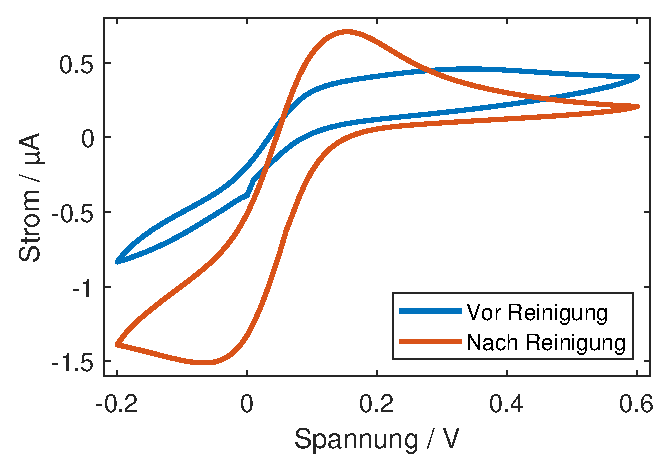
\includegraphics[trim=0 0 0 0,clip,width=\linewidth]{plot/CV_180um.eps}
\subcaption{CV vor und nach dem Reinigungszyklus}
\label{fig:CV}
\end{subfigure}
\caption{Elektrochemische Charakterisierung der Elektrode 13 unter einem Passivierungslayer mit \SI{180}{\micro\meter} Breite}
\label{fig:180um_ElChem}
\end{figure}

Die kurzgeschlossenen Elektroden produzierten im CV einen charakteristischen Peak bei \SI{0.9}{\volt} während der Reinigung. Die Entfernung des Mikrofilms ist außerdem für die Vergrößerung der Hysteresenfläche verantwortlich.(Abb. \ref{fig:CV_reinigung})
Die geringere Impedanz nach der Reinigung (Abb. \ref{fig:EIS}) zeigt zusätlich die Entfernung des vorhandenen Mikrofilms auf den einzelnen Elektrode 13 durch die Schwefelsäure. In einem CV nach der Reinigung (oranger Graph, Abb.\ref{fig:CV}) zeigen sich außerdem im Ansatz charakteristische Peaks in der Hysterese. Die - qualitativ - selben Werte ergeben sich ebenfalls für die Messungen mit Passivierungsstrukturen, die \SIlist{30;60}{\micro\meter} breiter sind.

\subsection{Flussratensensor}
Mit den fertig assemblierten Sensoren aus passiviertem Sensorchip und Mikrofluidik wurde dann versucht durch EIS eine Korrelation der Impedanz zur Flussrate zu finden. Dazu wurden bei unterschiedlichen Drücken Impedanzspektrogramme erstellt und in Matlab ausgewertet. Qualitativ ist ein leichter Trend zu erkennen, der jedoch nicht signifikant ist. 

\begin{figure}[!h]
    \centering
    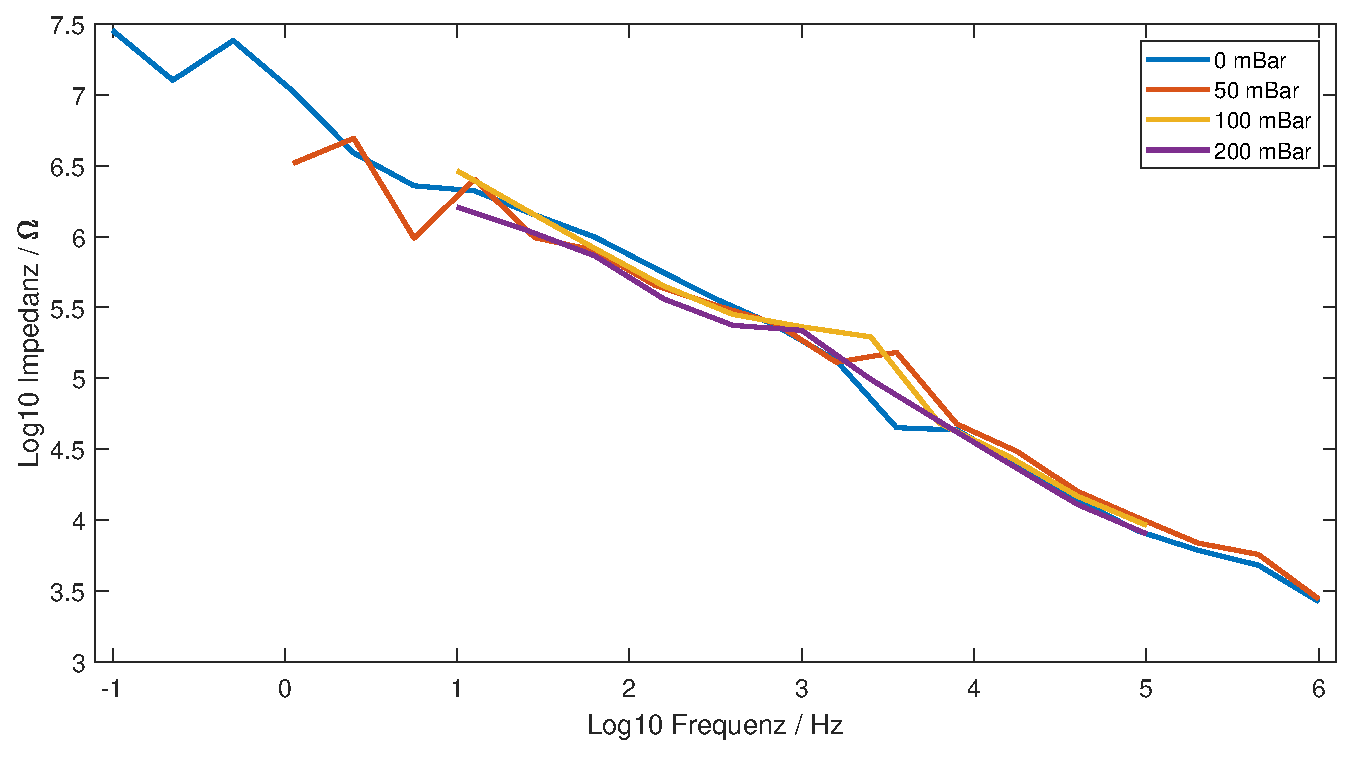
\includegraphics[width=\linewidth]{plot/FlowRate.eps}
    \caption{EIS bei verschiedenen Flussraten von \SI{20}{\milli\Molar} KCl}
    \label{fig:FlowRate}
\end{figure}
\clearpage

\begin{figure}[!h]
    \centering
    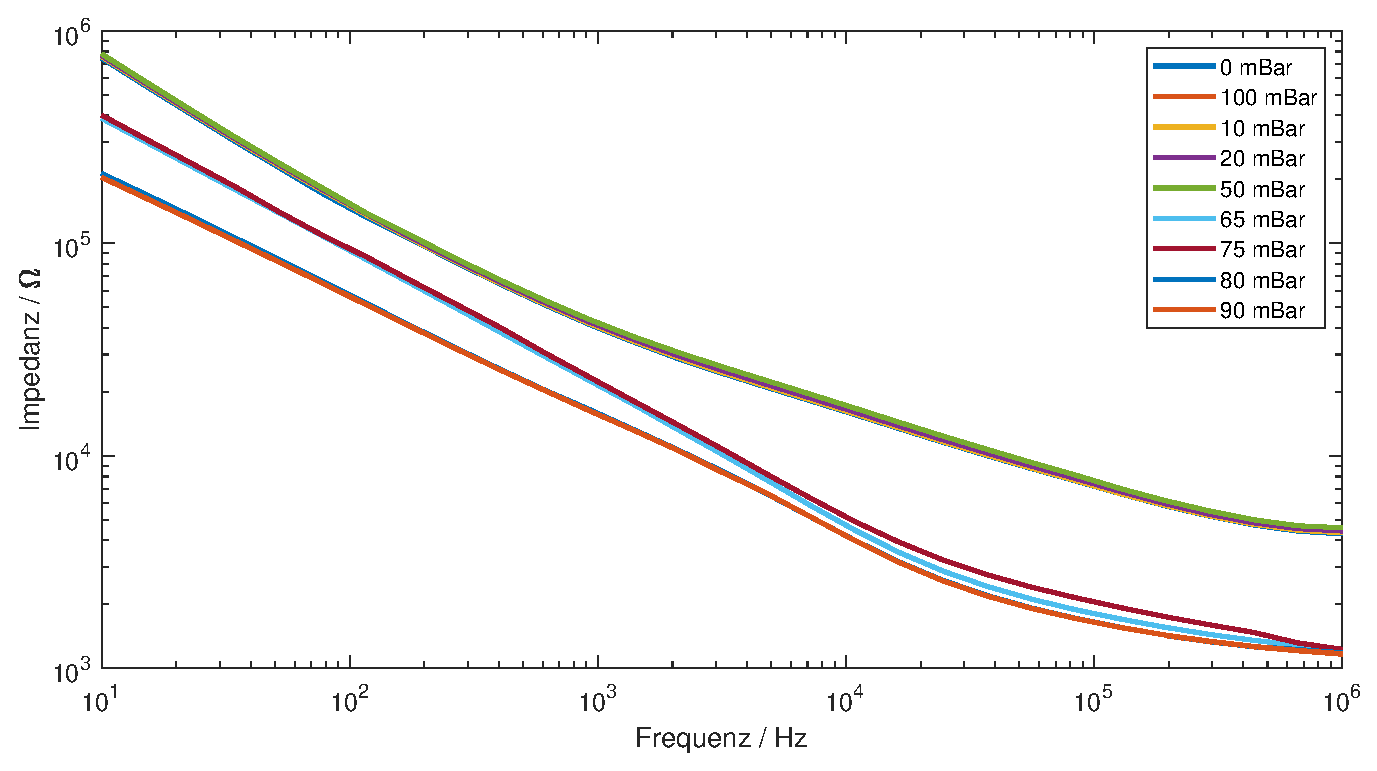
\includegraphics[width=\linewidth]{plot/FlowRate_fine.eps}
    \caption{EIS bei verschiedenen Flussraten von \SI{20}{\milli\Molar} KCl}
    \label{fig:FlowRate_fine}
\end{figure}



 \subsection{3D-Druck der Elektrodenstrukturen}
 Die PVP-AgNP-Elektroden aus dem parallel gelaufenen 3D-Druck wiesen einige Schwachstellen auf.  Auf dem Foto (Abb. \ref{fig:inkjet}) sind bereits einige schwarze Stellen auf den Silberstrukturen sichtbar, an denen die Tinte ungünstig verlaufen ist bzw. gedruckt wurde. Dies lässt sich auf die Oberflächenspannung der Tinte selbst und die Überlappung bzw. den Ausfall einiger Nozzles zurückführen. 
 \begin{figure}[!htb]
     \centering
     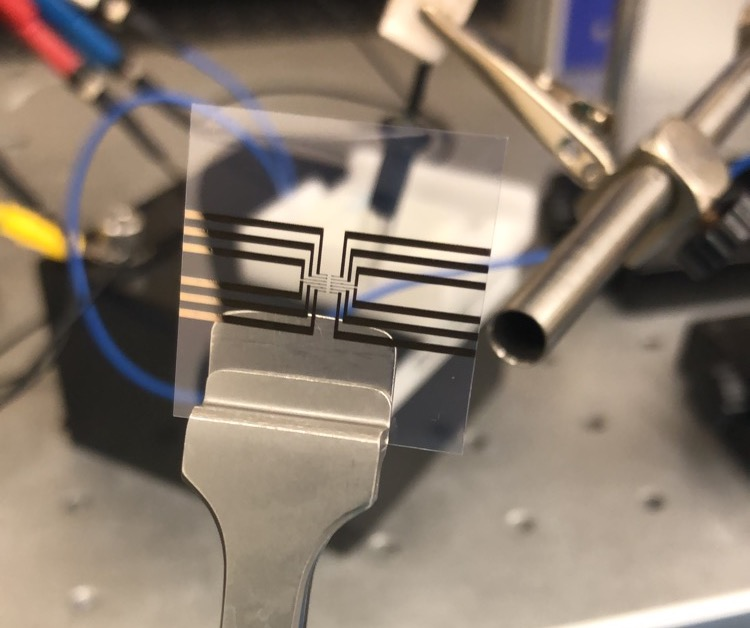
\includegraphics [trim=100 200 200 100,clip,width=.5\linewidth]{img/inkjet_chip.jpeg}
     \caption{Gedruckte Silberelektroden aus dem Inkjet-3D-Drucker.}
     \label{fig:inkjet}
 \end{figure}

\subsection{Galvanisierung der Silberelektroden}
Die fertig prozessierten Silberelektroden wurden nun mit Goldcyanid galvanisiert, um die Cytokompatibilität zu gewährleisten. Nach einigen Ablösungen des Goldes von den Elektroden bzw. einem allgemein schlechten Galvanisierungsergebnis, wurde das  Reduktionspotential von \SI{-1.0}{\volt} auf \SI{-0.9}{\volt} verringert, was zuverlässigere Beschichtungen lieferte.

\subsection{Aerosoldruck der Pillar-Strukturen}
Im Anschluss wurde auf die galvanisierten Elektroden PEDOT:PSS Pillars mittels Aerosol-Jetting gedruckt. Nach der Bestimmung passender Drücke im Scher-, Absaug- und Atomisierungsstrom, wurden auf die Feedlines Pillarstrukturen mit \SI{30}{\micro\meter} Höhe gedruckt.